\documentclass[journal,twoside]{IEEEtran}
\IEEEoverridecommandlockouts
% The preceding line is only needed to identify funding in the first footnote. If that is unneeded, please comment it out.
\usepackage{cite}
\usepackage{hyperref}
\usepackage{natbib}
\usepackage{booktabs}
\usepackage{threeparttable}
\usepackage{amsmath,amssymb,amsfonts}
\usepackage{algorithmic}
\usepackage{graphicx}
\usepackage{textcomp}
\usepackage{xcolor}
\makeatletter
\def\UrlAlphabet{%
      \do\a\do\b\do\c\do\d\do\e\do\f\do\g\do\h\do\i\do\j%
      \do\k\do\l\do\m\do\n\do\o\do\p\do\q\do\r\do\s\do\t%
      \do\u\do\v\do\w\do\x\do\y\do\z\do\A\do\B\do\C\do\D%
      \do\E\do\F\do\G\do\H\do\I\do\J\do\K\do\L\do\M\do\N%
      \do\O\do\P\do\Q\do\R\do\S\do\T\do\U\do\V\do\W\do\X%
      \do\Y\do\Z}
\def\UrlDigits{\do\1\do\2\do\3\do\4\do\5\do\6\do\7\do\8\do\9\do\0}
\g@addto@macro{\UrlBreaks}{\UrlOrds}
\g@addto@macro{\UrlBreaks}{\UrlAlphabet}
\g@addto@macro{\UrlBreaks}{\UrlDigits}
\makeatother
\def\BibTeX{{\rm B\kern-.05em{\sc i\kern-.025em b}\kern-.08em
    T\kern-.1667em\lower.7ex\hbox{E}\kern-.125emX}}
\pagestyle{headings}
\markboth{Bioinformatics. Specialty  Innovation  and  Entrepreneurship  Training 2021}
{Zhao. A Weight Array Model for Prediction of Eukaryotic Genetic Splice Sites (June 2021)}
\begin{document}

\title{WAM: A Weight Array Model for Prediction of Eukaryotic Genetic Splice Sites\\
}

\author{\IEEEauthorblockN{1\textsuperscript{st} Ziwen Zhao} \\
\IEEEauthorblockA{\textit{College of Life Science and Technology} \\
\textit{Huazhong University of Science and Technology}\\
Wuhan, China \\
justn582@gmail.com}
}

\maketitle

\begin{abstract}
Splice sites are a vitally important gene sequence pattern amongst the functional sites inside a eukaryotic gene. However, splice site prediction does not come easy thanks to the extreme complexity of human genome. In this paper, an optimized frequency-based method to predict eukaryotic genetic splice site patterns with the Weight Array Model (WAM) is proposed, which is a feasible lightweight computational approach for gene functional site finding, in order to deal with splice site predictions. We prove its accuracy and high efficiency by comparison studies on the renowned Kulp \& Reese human genome dataset, during which we achieve excellent results on several different metrics. The source code is available on GitHub and can be obtained from \url{https://github.com/Newiz430/SplicePredictor}. 
\end{abstract}

\begin{IEEEkeywords}
splice site, weight array, statistics, frequency-based, probability matrix
\end{IEEEkeywords}

\section{Introduction}\label{1}

\IEEEPARstart{G}{ene} finding by computational methodologies, the foundation for all further investigation in functional genomics, has attracted considerable research attention since the 20\textsuperscript{th} century \cite{burge1997prediction}. With the thriving of functional genomics after the completion of Human Genome Project (HGP), functions of the elements of eukaryotic gene sequences were beginning to surface. Researchers came to realize that DNA sequences, other than genes, contain a huge amount of information, most of which is correlated with the structural features of nucleic acids and in general determines the DNA - protein, or DNA - RNA interactions. Such information is mostly provided by a variety of functional sites (i.e. sequence motif). The splice sites are a vitally important eukaryotic gene sequence pattern amongst all these sites. As terminal points of RNA splicing, splice sites label the junction of transcript exons and introns, assisting biologists in identifying and positioning the coding sequence within a gene. Splicing, itself, also influences the structure and function of genes, which makes genes more ``modular'', allowing new combinations of exons to be created during evolution. Furthermore, new exons can be inserted into old introns, creating new proteins without disrupting the function of the old gene \cite{clancy2008rna}. Hence the discovery and prediction of splice sites are of great significance for genetic selective expression research. 

\begin{figure}[htbp]
\centerline{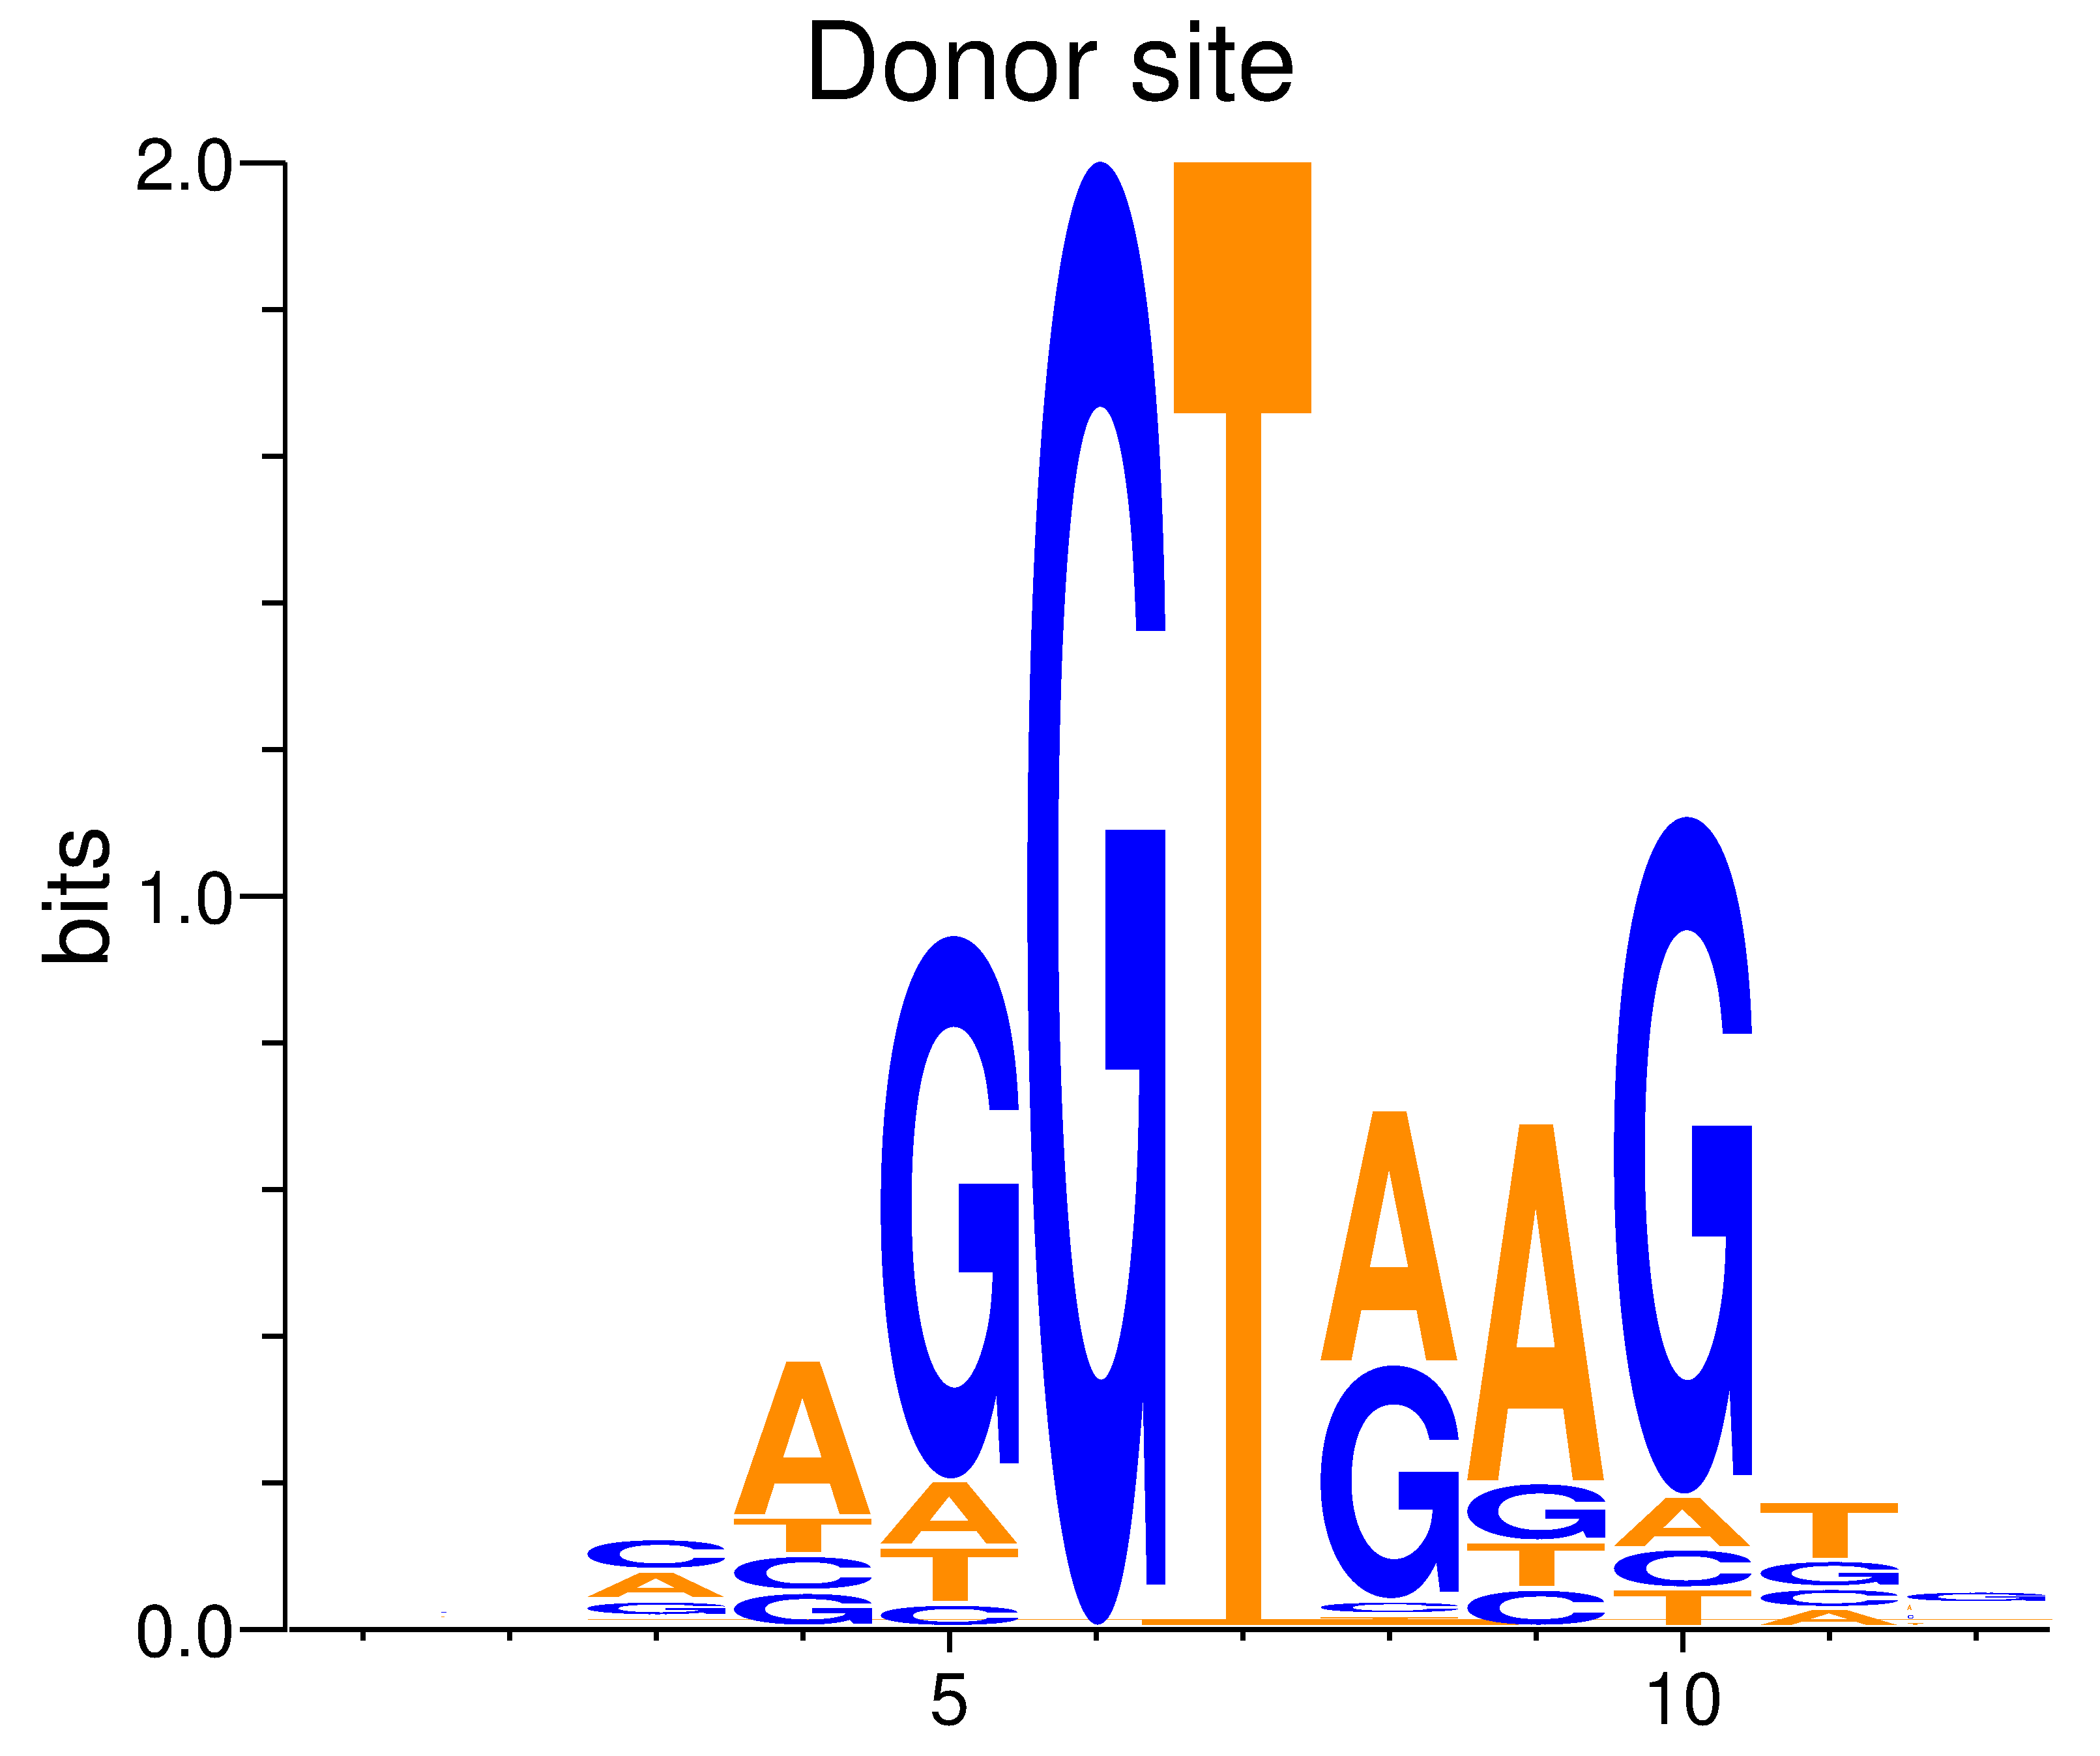
\includegraphics[scale=0.85]{Pics/donor_logo.png}}
\centerline{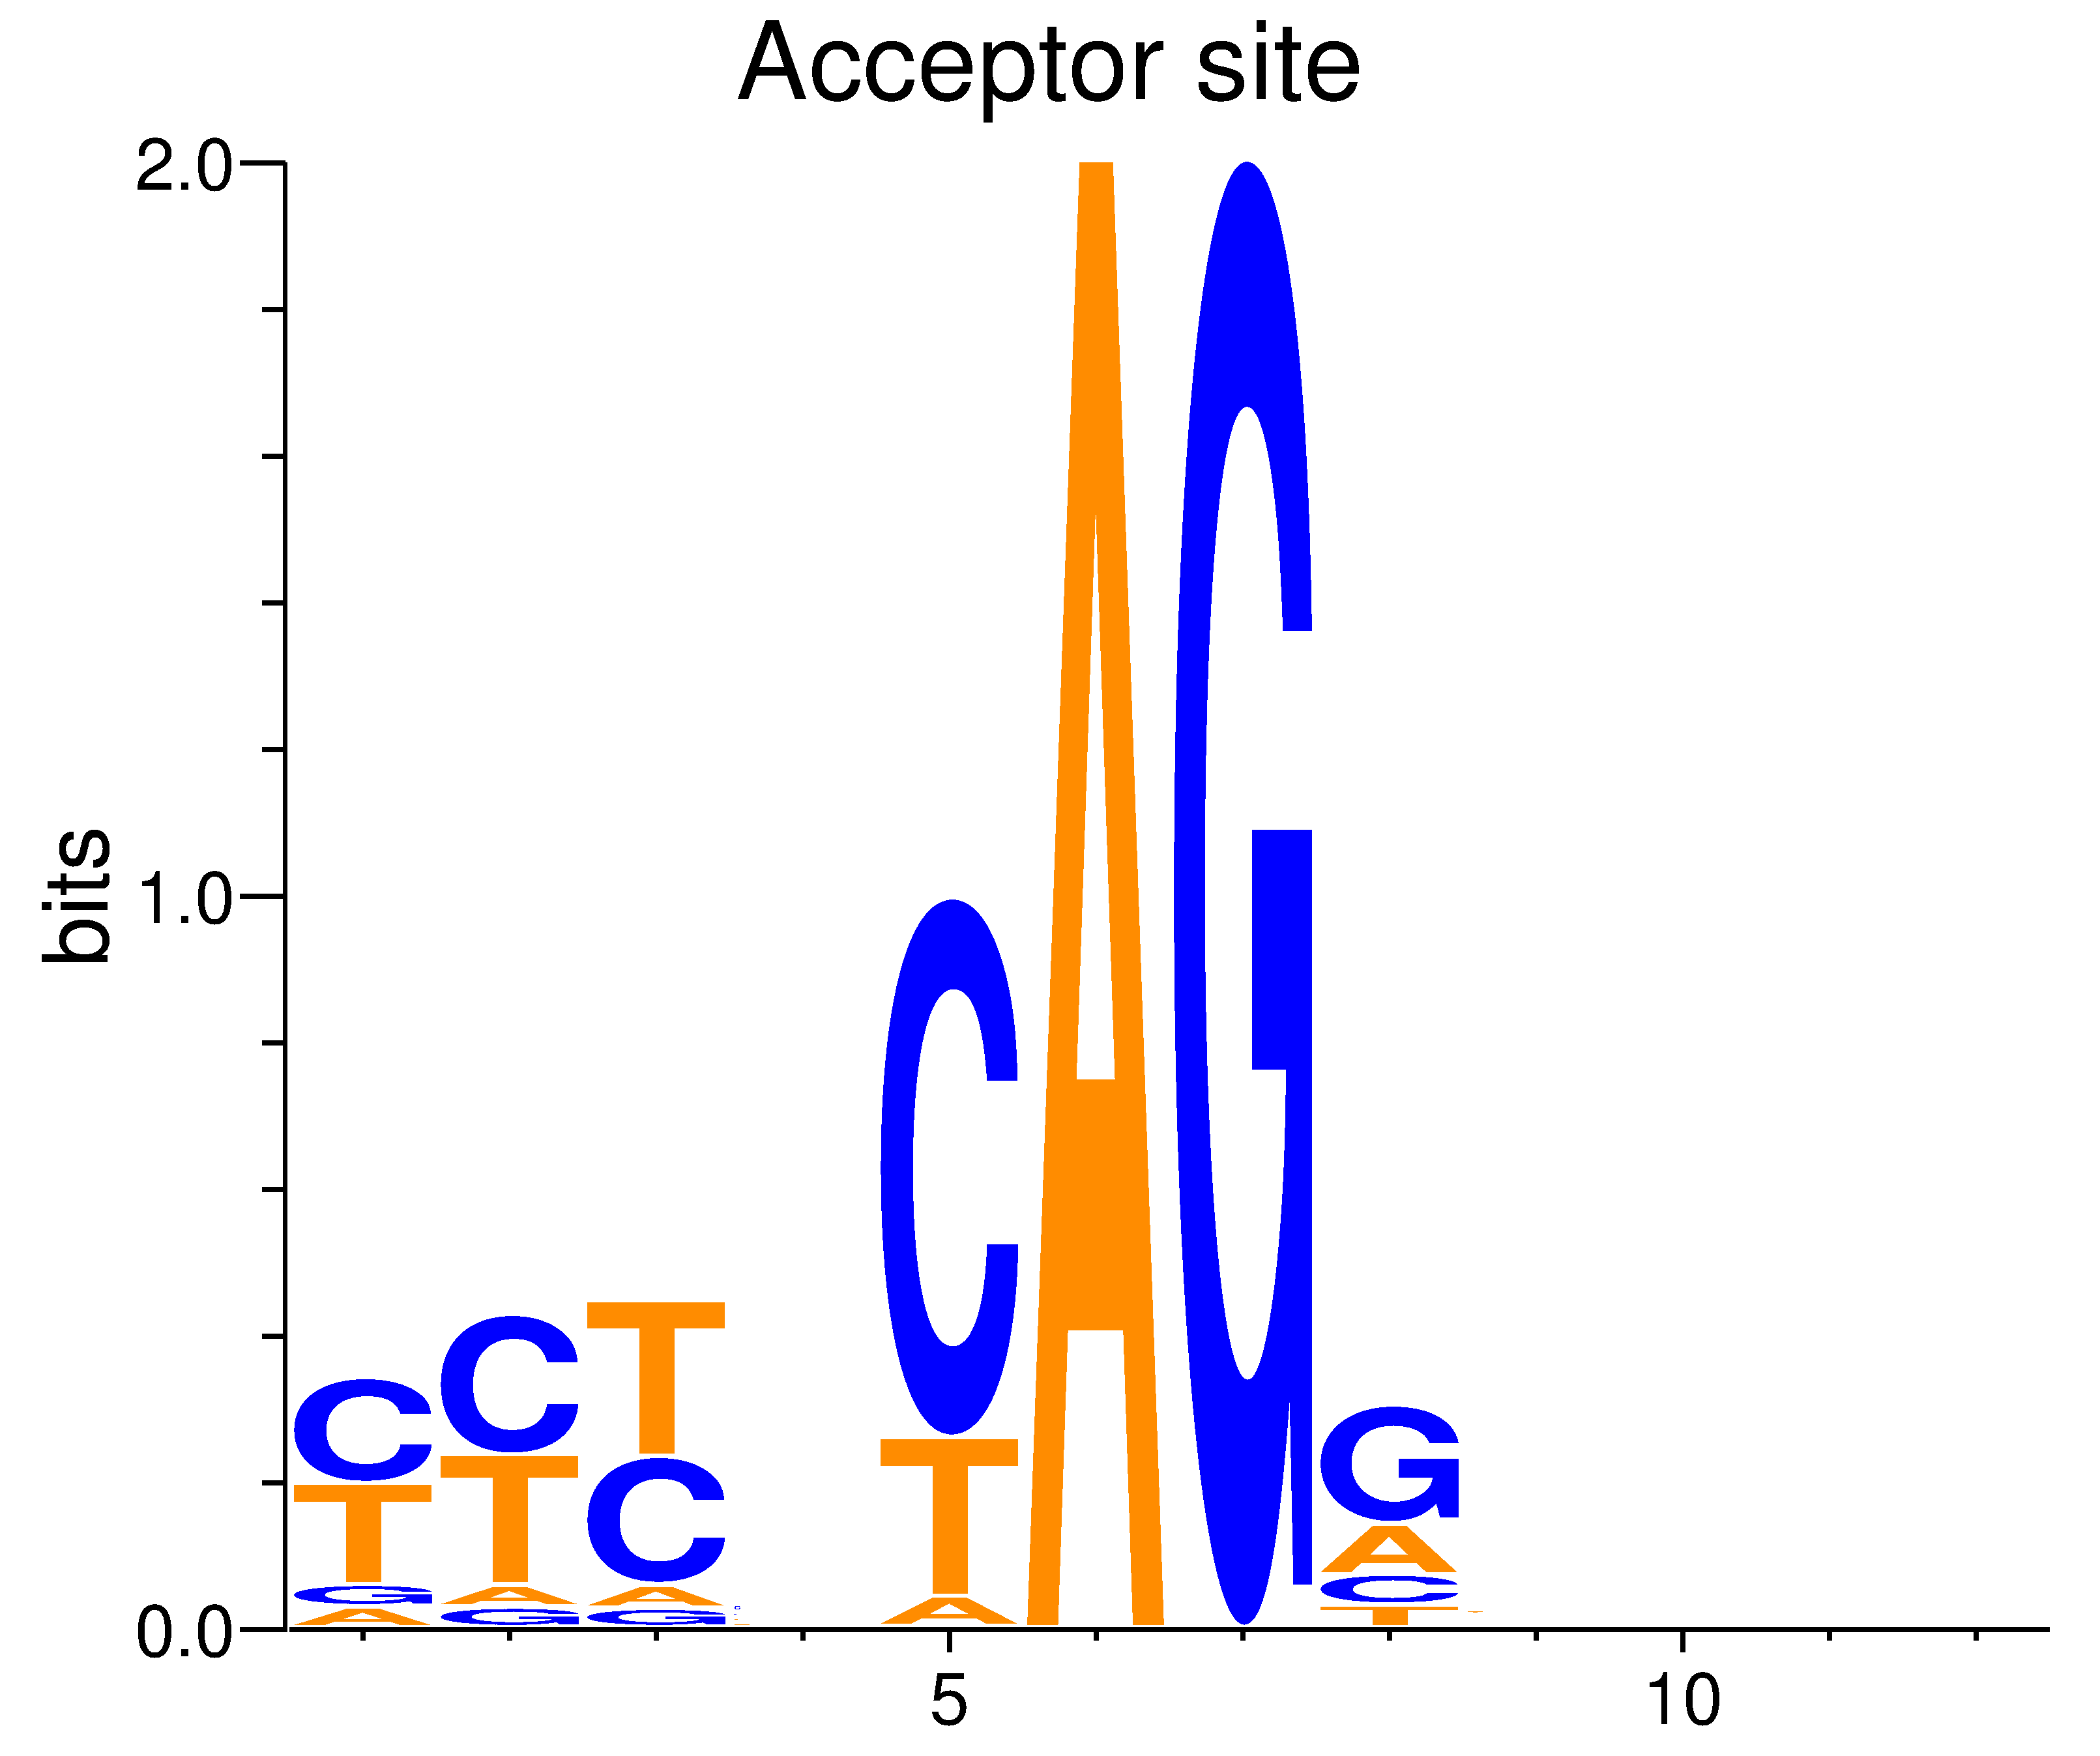
\includegraphics[scale=0.85]{Pics/acceptor_logo.png}}
\caption{Base distribution represented as sequence logos \cite{schneider1990sequence} for eukaryotic gene splice sites (5 upstream sites, 2 conservative sites \& 5 downstream sites): \textbf{top}, donor site; \textbf{bottom}, acceptor site. The most conserved sites is revealed within logo pictures: for donor sites, GT (6, 7); acceptor sites, AG (6, 7). Despite these two, distribution of adjacent sites (5, 8, 9, 10 for the donor, 5 for the acceptor) appear to have some consistency, too. The polypyrimidine tract can also be observed upstream of the acceptor site (1, 2, 3). The information content at a certain point $R_i$ is given by $R_i = \log_24 - (H_i + e_n)$ where $H_i = -\sum\limits_{i=1}^4{P_i(\log_2{P_i})}$ is the Shannon entropy \cite{shannon1948mathematical}, using bit as the basic unit. Higher the bits, higher the relative frequency of that base \cite{schneider1986information}. }
\label{fig1}
\end{figure}

A splice site locates in the edge of an intron, including a donor site (5' end of the intron) and an acceptor site (3' end of the intron). As a typical sequence motif, the donor site includes an almost invariant sequence GU at the 5' end of the intron, within a larger, less highly conserved region. The splice acceptor site at the 3' end terminates the intron with an almost invariant AG sequence \cite{black2003mechanisms}.  Some sections of the intron foretell the positions of these two sites. For example, a fragment of sequence upstream of the acceptor consisting of cytosines and thymines, which is called a polypyrimidine tract \cite{lodish2008molecular}. Fig. \ref{fig1} shows the base distributions adjacent of the splice donor sites and acceptor sites. 

As a matter of fact, accurate prediction does not come easy thanks to the extreme complexity of human genome. On one hand, the number and length of exons and introns in a eukaryotic gene exhibit great uncertainty. One eukaryotic gene contains 5.48 exons with 30 - 36 bps long on average. While the longest exon in the human genome is 11555 bp long, several exons have been found to be only 2 bp long \cite{sakharkar2004distributions}. On the other, the existence of alternate splicing make it harder to predict \cite{black2003mechanisms}. In this paper, we apply a Bayesian method for gene functional site finding to predict eukaryotic gene splice sites, and prove its feasibility. 

\subsection{Related Work}\label{1.1}

Several typical computational methods that attempt to predict eukaryotic splice sites from unknown gene sequences (i.e. \textsl{ab initio} prediction) have been proposed previously. 

Frequency-based methods count the nucleotide frequencies of each site via multiple sequence alignment, etc. and work out the log-odds ratio to compare and find conservative sections in the alignment results. Rodger, et al. (1983) \cite{staden1984computer} proposed a computational model using a weight matrix to represent each type of recognition sequence. A weight matrix is a two dimensional array of values that represent the score for finding each of the possible sequence characters at each position in the target signal. The Weight Matrix Model (WMM) now becomes deprecated owing to its poor accuracy and its independence assumption, that is, WMM only takes point-wise base distribution into consideration, regardless of the potential dependence between adjacent points which is more conformable to the realistic situations. 

Bayesian methods are ones that consider long range dependency among nucleotide sequences. Chen, et al. (2005) \cite{chen2005prediction} proposed a method using dependency graphs and its expanded form - Bayesian Network to fully capture the intrinsic interdependency between base positions in a splice site. The entire model, including the DAG structures and conditional probabilities, is learned \textsl{ab initio} from a training set. However, with astronomical computation complexity and model training difficulty, the performance of Bayesian models is not in keeping with them. 

Supervised learning methods learn a model from existing training set which is able to identify the most effective pattern automatically. Duan, et al. (2008) \cite{duan2008position} developed the support vector machine (SVM) for position-specific residue preference feature prediction which determines the second structure of double helices. Ryen et al. (2008) \cite{ryen2008splice} introduced the artificial neural network (ANN) in this area and trained the model with backpropagation, which can make predictions without prior knowledge of any sensor signals. Accurate and efficient learning approaches they are, supervised learning methods are heavily dependent on the mass and quality of training sets. Models may not be improved and a computational resource waste may happen when an unbalanced dataset or one with too many noises is provided. For SVMs, kernel function selection is a tricky problem, and neural networks acquire a suitable framework and initial hyperparameters. 

\subsection{Contributions}\label{1.2}

In this work, we propose an optimized frequency-based method to predict splice site patterns with the weight array model. At bottom, a weight array method continues to extract splice signals, count the frequencies of nucleotides and fill the matrices, identical with WMM. What we can use to distinguish WAM from WMM is that WAM takes into account the correspondence between current position and an adjoining position, which we certify conducive to promote accuracy of splice site prediction. Our contributions are listed as follows. 

\begin{itemize}
\item We implemented the weight array model by Python using the given KR set and estimated its performance on the BG set, referring to the existing experiment by Zhang et al. (1993) \cite{zhang1993weight}.
\item We did a comparison study between WMM and WAM model to prove the superiority of our model. 
\item We applied our model on the prediction of both donor splice sites and acceptor splice sites. 
\end{itemize}

\begin{figure*}[htbp]
\centerline{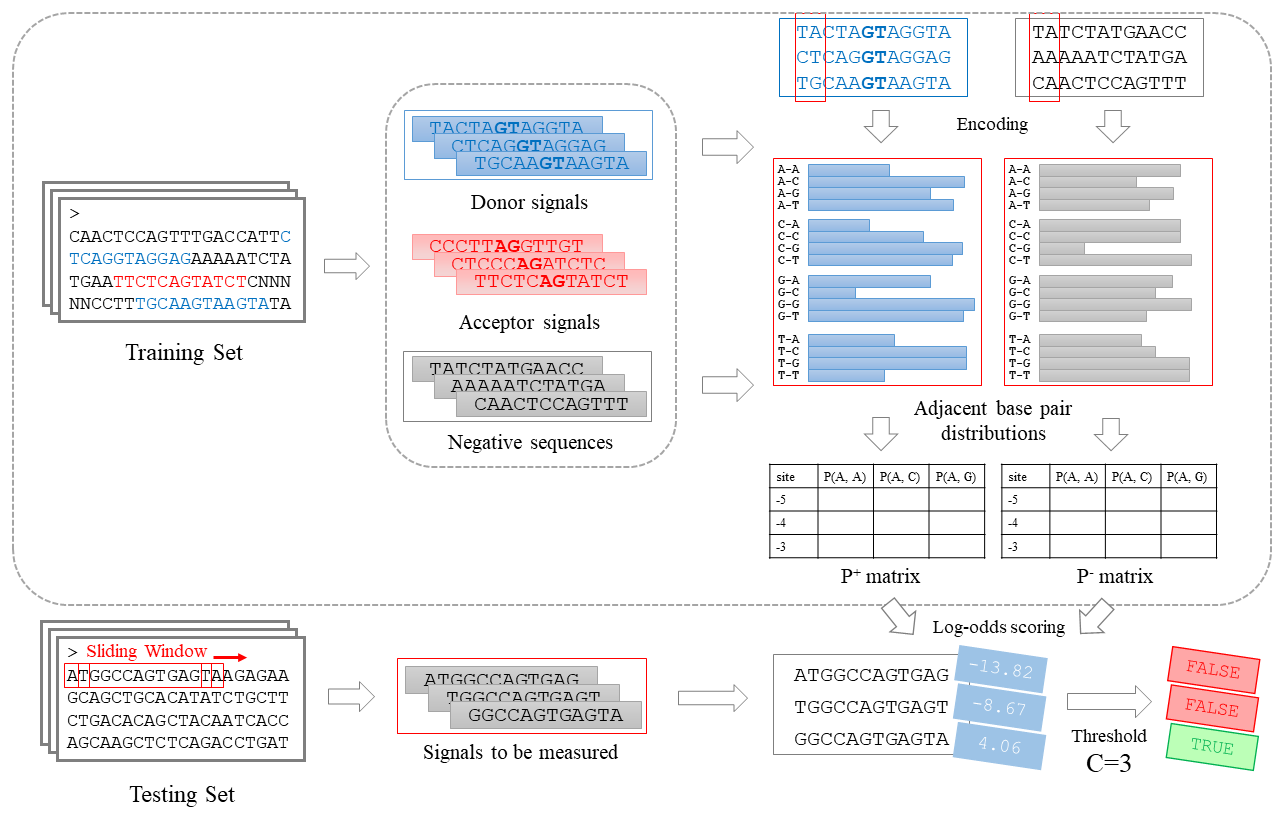
\includegraphics[scale=0.5]{Pics/WAM.png}}
\caption{Overall architecture of the WAM splice predictor. We use the training set to create two matrices by these steps: extracting positive site signals \& randomly choosing negative signals, encoding \& counting the bases for each position, calculating distribution probabilities, filling the matrices and saving for future predictions. We use P matrices to predict unknown signals by these steps: extracting testing sequences of same length by window-sliding, scoring the sequences position-wise with obtained probabilities, calculating the binary log-odds scores, and comparing them with a given threshold to make final judgment. }
\label{fig2}
\end{figure*}

\section{Methods}\label{2}

Our method is illustrated in Fig. \ref{fig2}, which mainly contains two parts. The statistics of base pair distribution is carried out at the ``training'' step, and sequences of the testing set are scored by probability matrices at the ``predicting'' step. See below for more detailed presentation. 

\subsection{Hypothesis}\label{2.1}

WAM is suitable for predicting work only when the two assumptions below stand. Firstly, we assume conservation around the functional splice sites through the entire experiment. Additionally, we consider the intrinsic interdependency only exists between adjacent sites. As for data, we assume that everything about the splice site pattern remained unknown (including the obligatory sites GT / AG) until we dug them out, in order to guarantee the generality of our model, since our aim is to make it possible to branch out to other unidentified functional sites. 

\subsection{Data Extraction}\label{2.2}

Dash et al. (2001) \cite{dash2001modeling} found in predicting splice sites by a Bayesian network that it achieves better performance when both of the upstream and downstream feature lengths are greater than 15. With a view to simplifying model and decreasing the computation, we choose 5 upstream sites and 7 downstream sites of intron / exon junctions to form 12 nt long signal sequences from the primary training set. We abandon sequences containing ambiguous bases, whose correspondence with the splice sites we consider inapparent. The training set provides 2,381 donor signals and 2,381 acceptor signals. As for negative samples, Chen, et al. \cite{chen2005prediction} used pseudo splice sites as false data, extracted by searching for negative sample sequences with $P_{+1}P_{+2} = \text{GU / AG}$ whereas, according to the splice site hypothesis above, We randomly selected about 5,000 sites in sections which do not intersect with all donor and acceptor sites, and combined with positive ones to get actual training dataset, the positive-negative ratio of which is about 1:2. Additionally, we export sequences with the same length by window sliding from the primal testing set and build the actual testing set in a positive-negative ratio of 1:20.

\subsection{Construction of Probability Matrices}\label{2.3}

For convenient computing, we encode the extracted sequences. We use 0, 1, 2, and 3 to represent bases A, C, G, T which indicates the position in the P matrices of each base. For positive samples with the length of $\lambda$, we create a $\lambda$ * 4 * 4 probability matrix $P^+$, in which each position  $(N_j, N_{j+1})$ of the $i$th 4 * 4 submatrix stores the conditional probability $P^+[i, N_j, N_{j+1}]$ which denotes the probability of $N_j$ at the current position $j$ if the nucleotide at position $j+1$ is $N_{j+1}$. Each probability is calculated by counting the frequencies of every situations $\text{freq}(i, N_j, N_{j+1})$ in the positive samples and expressed as
\begin{equation}
P^+[i, N_j, N_{j+1}] = \displaystyle\frac{\text{freq}(i, N_j, N_{j+1})}{\sum\limits_{N_{j+1}}\text{freq}(i-1, N_j, N_{j+1})}
\label{eq1}
\end{equation}
with
\begin{equation}
i = 2, 3, \cdots, \lambda, \ \ j = 1, 2, 3, 4. \notag
\end{equation}

The conditional distribution probabilities of negative samples $P^-[i, N_j, N_{j+1}]$ are defined likewise: 
\begin{equation}
P^-[i, N_j, N_{j+1}] = \displaystyle\frac{\text{freq}(i, N_j, N_{j+1})}{\sum\limits_{N_{j+1}}\text{freq}(i-1, N_j, N_{j+1})}.
\label{eq2}
\end{equation}
Then we put the base distribution probabilities of the first position $P^+[1, N]$ into 1D-arrays $P_0^+$ and $P_0^-$ : 
\begin{equation}
P_0^+[1, N_j] = \displaystyle\frac{\text{freq}(1, N_j)}{\sum\limits_{N_{j}}\text{freq}(1, N_j)}
\label{eq3}
\end{equation}
\begin{equation}
P_0^-[1, N_j] = \displaystyle\frac{\text{freq}(1, N_j)}{\sum\limits_{N_{j}}\text{freq}(1, N_j)}
\label{eq4}
\end{equation}

\begin{figure*}[htbp]
\centerline{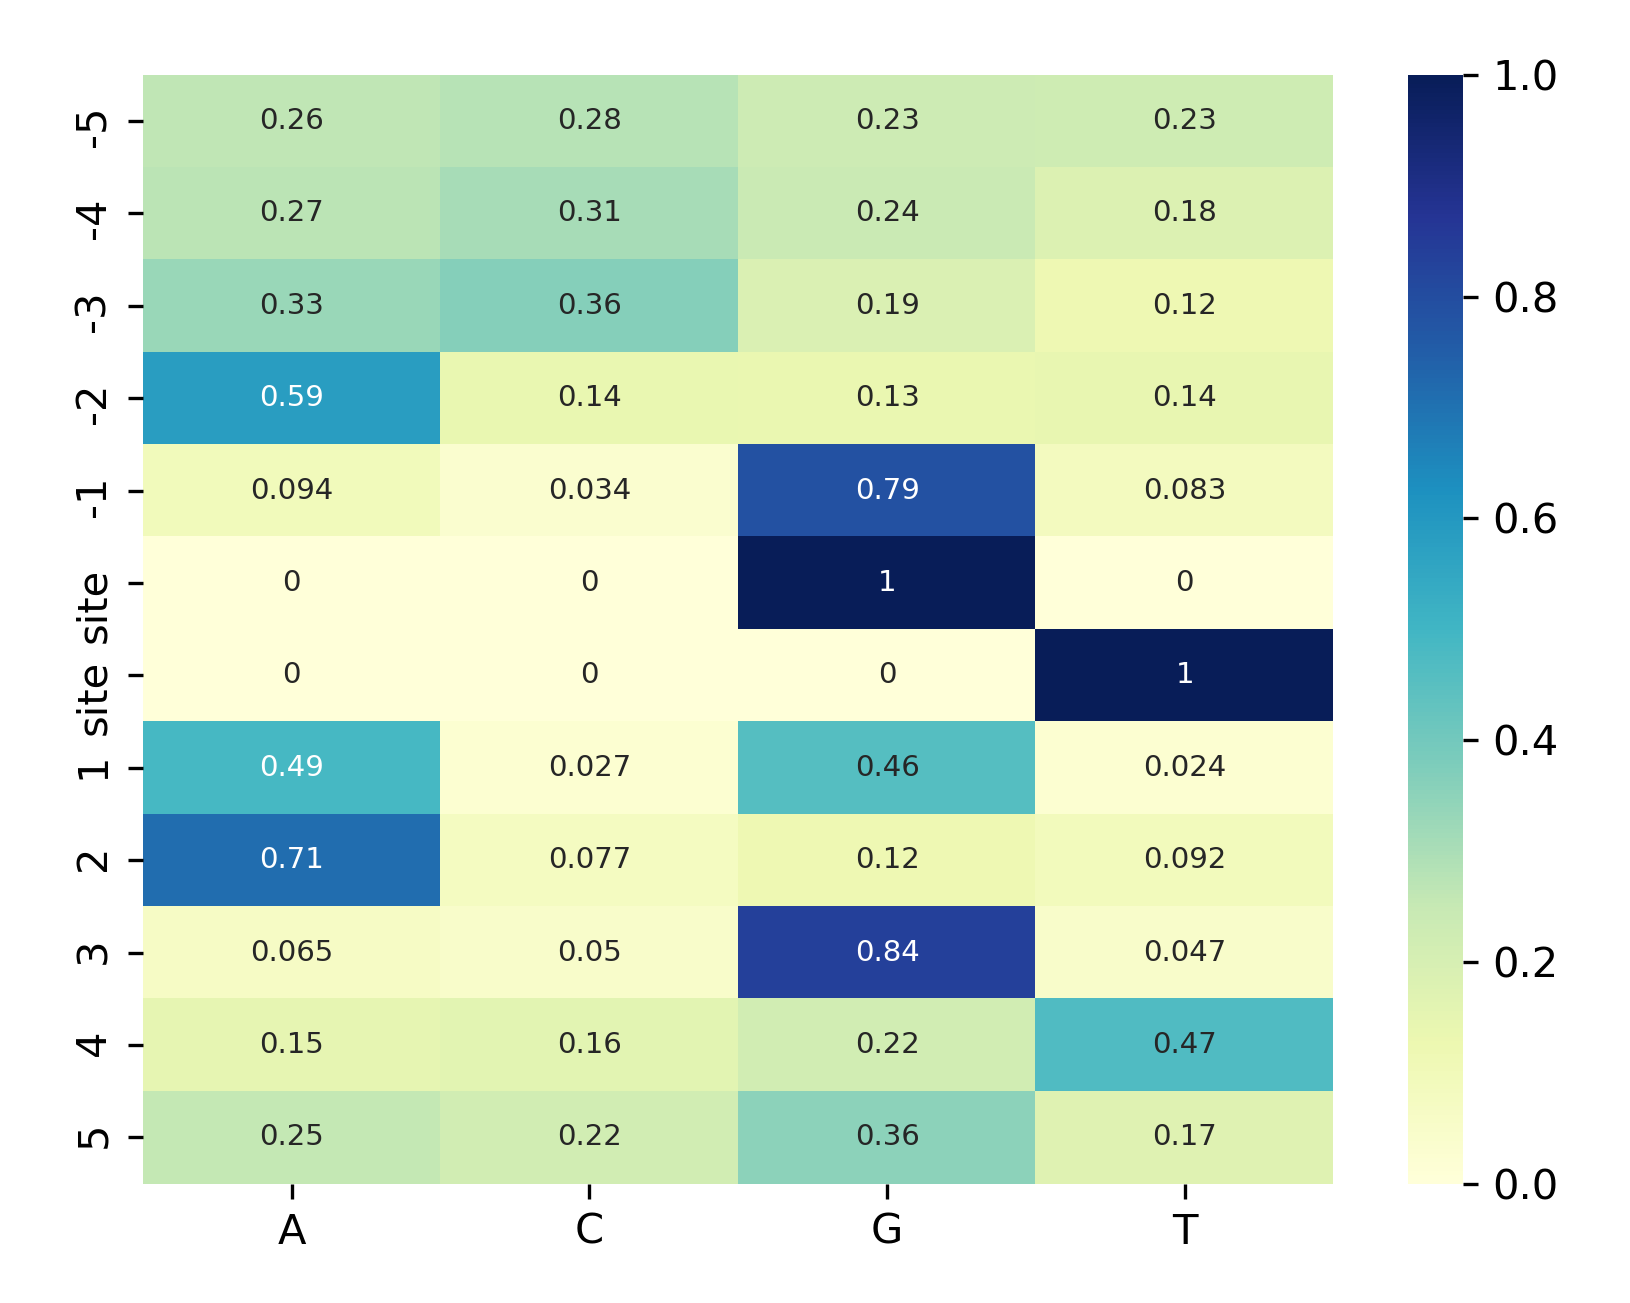
\includegraphics[scale=0.6]{Pics/ssheatmap_donor.png}
    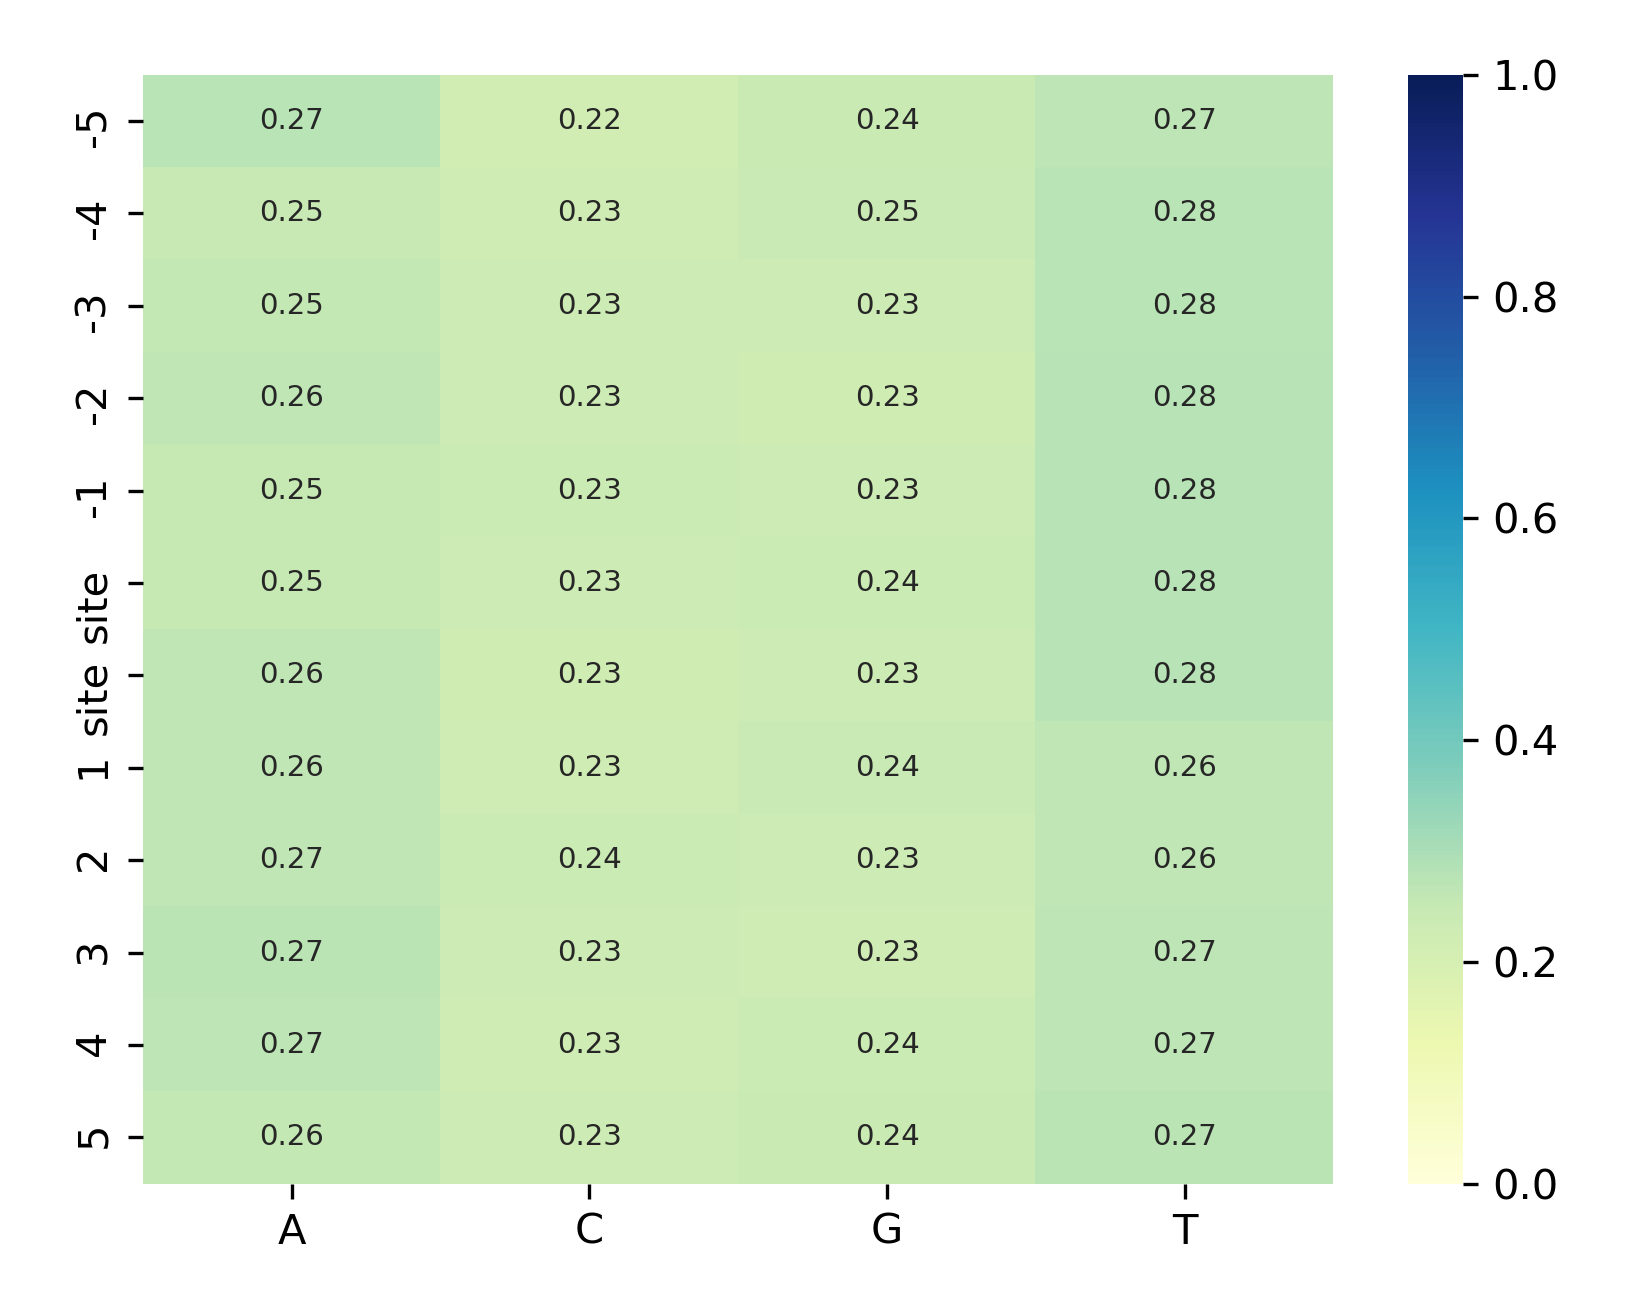
\includegraphics[scale=0.6]{Pics/ssheatmap_neg.png}}
\centerline{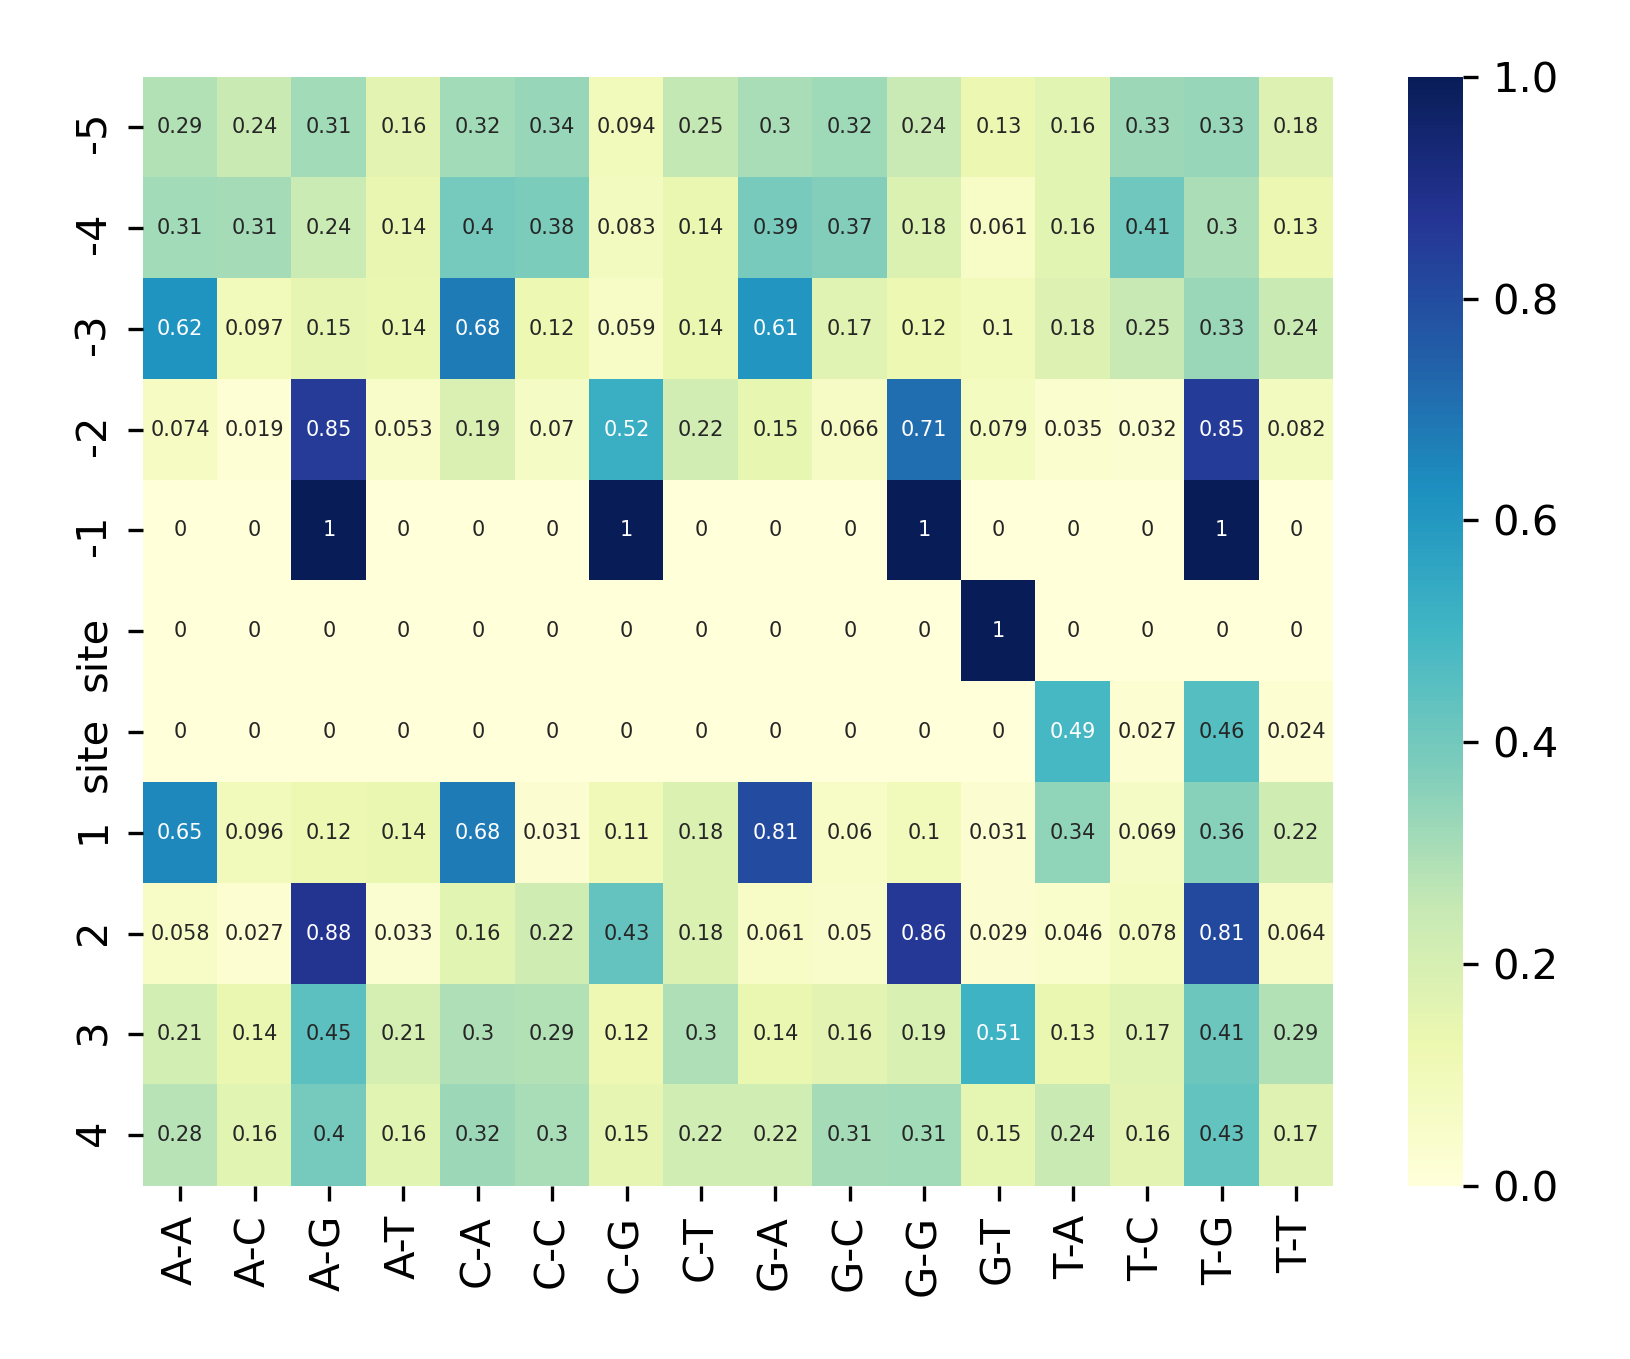
\includegraphics[scale=0.6]{Pics/asheatmap_donor.png}
    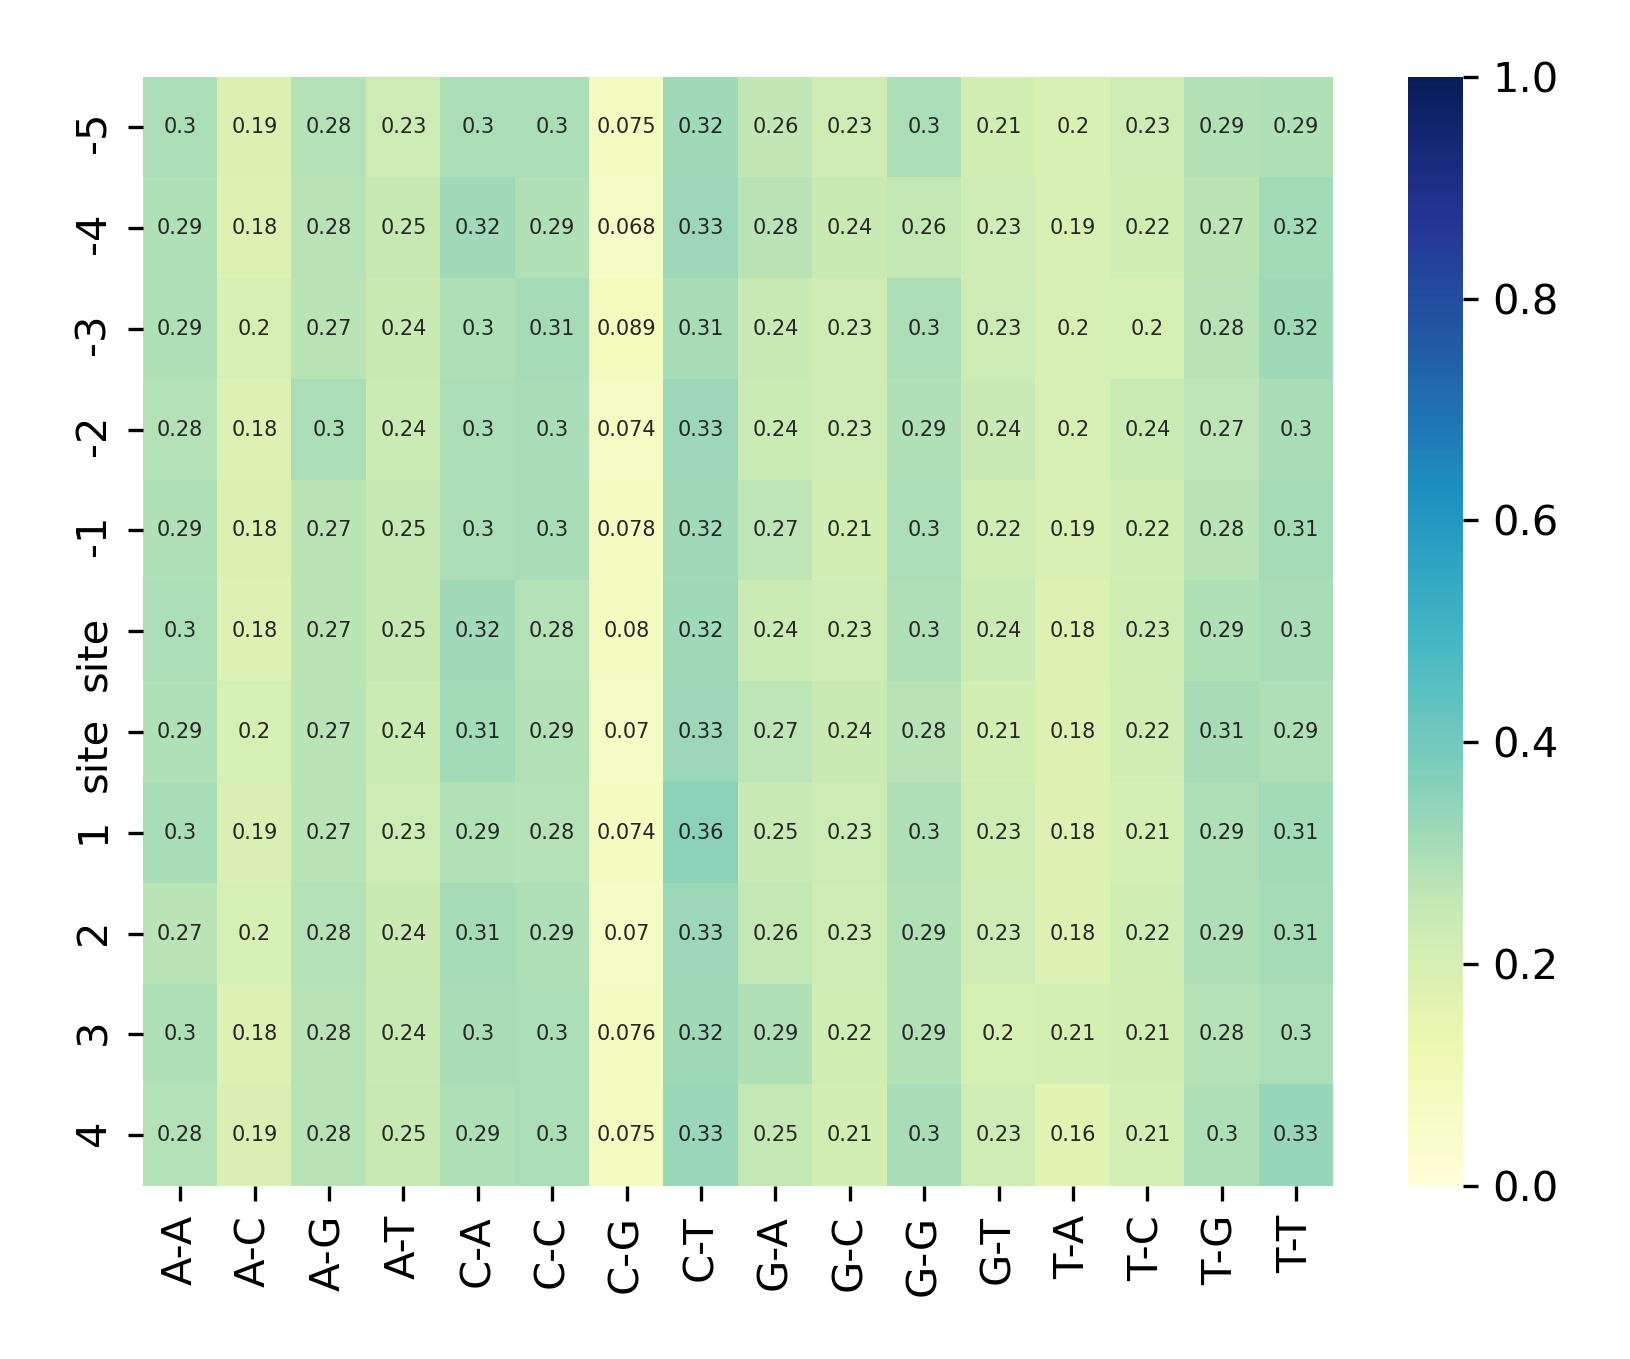
\includegraphics[scale=0.6]{Pics/asheatmap_neg.png}}
\centerline{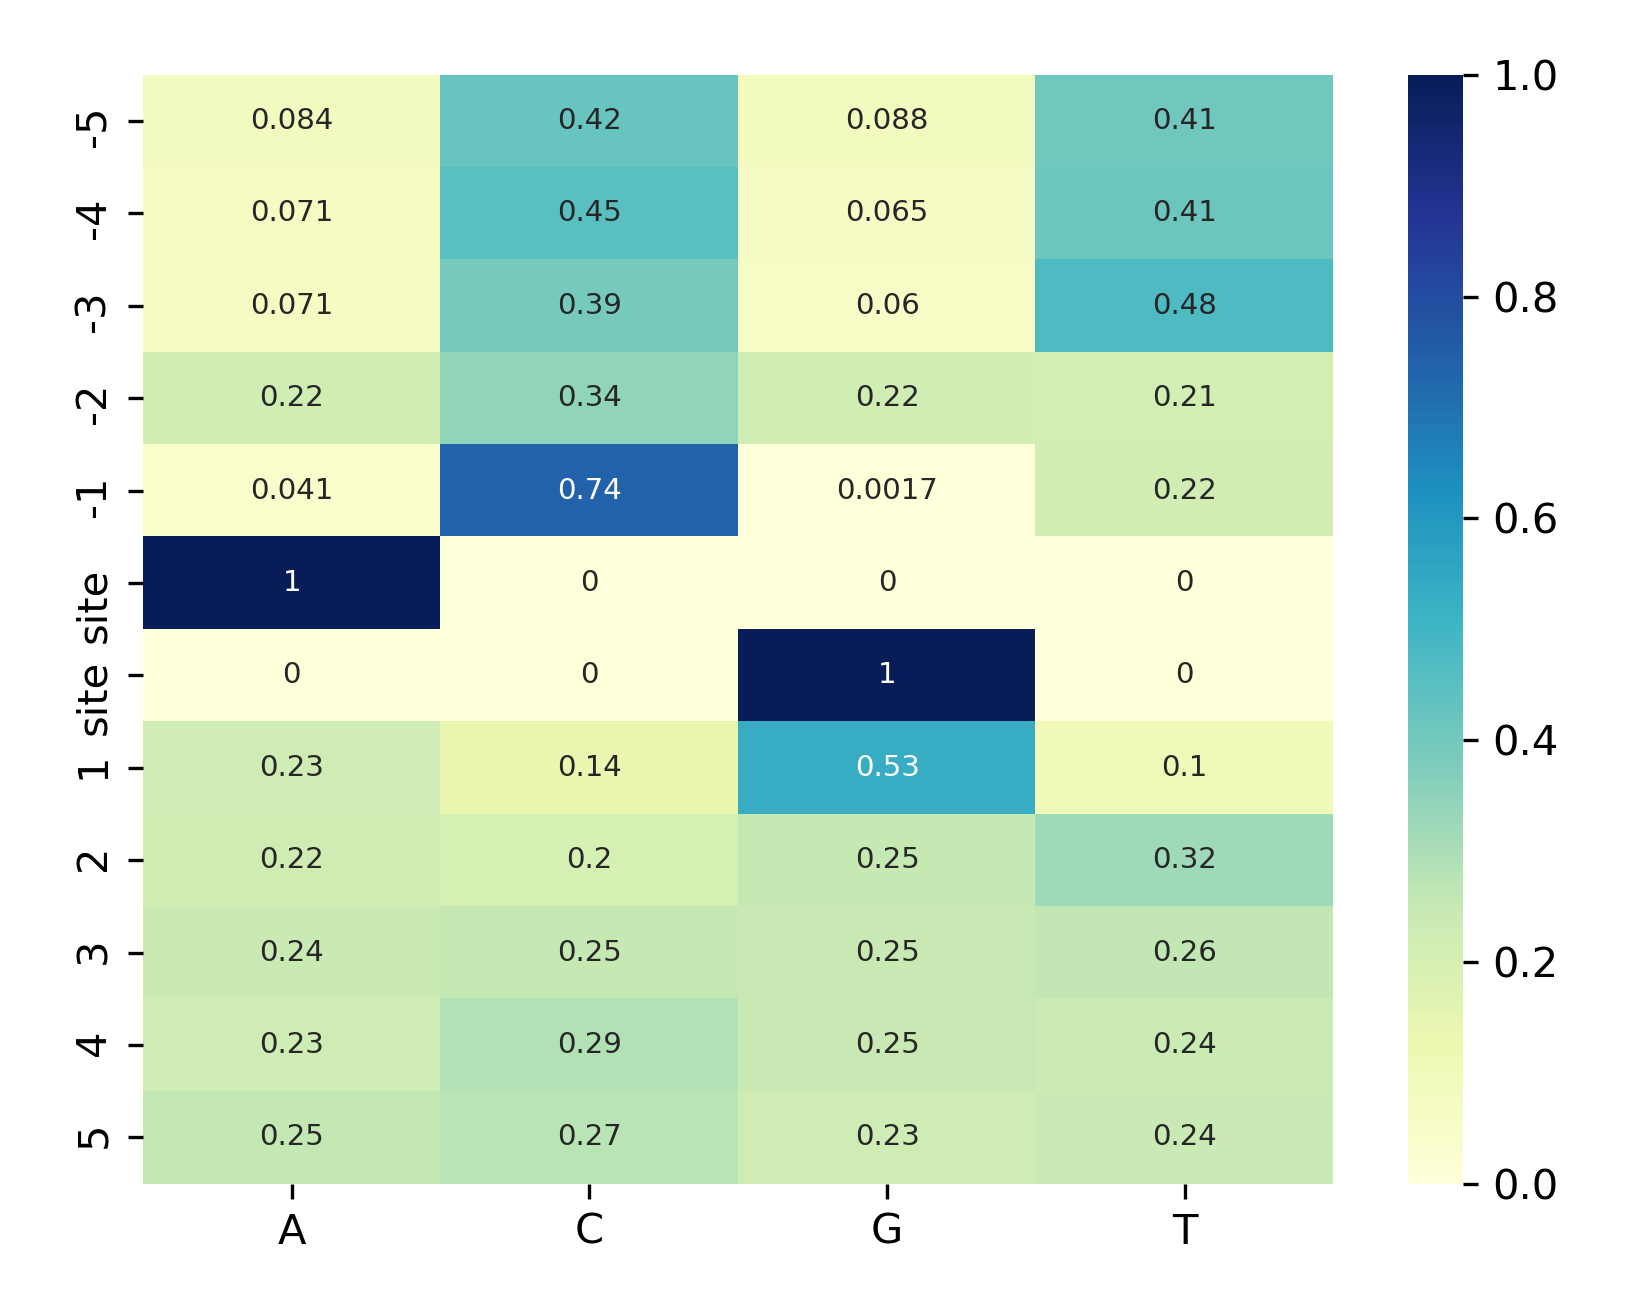
\includegraphics[scale=0.6]{Pics/ssheatmap_acceptor.png}
    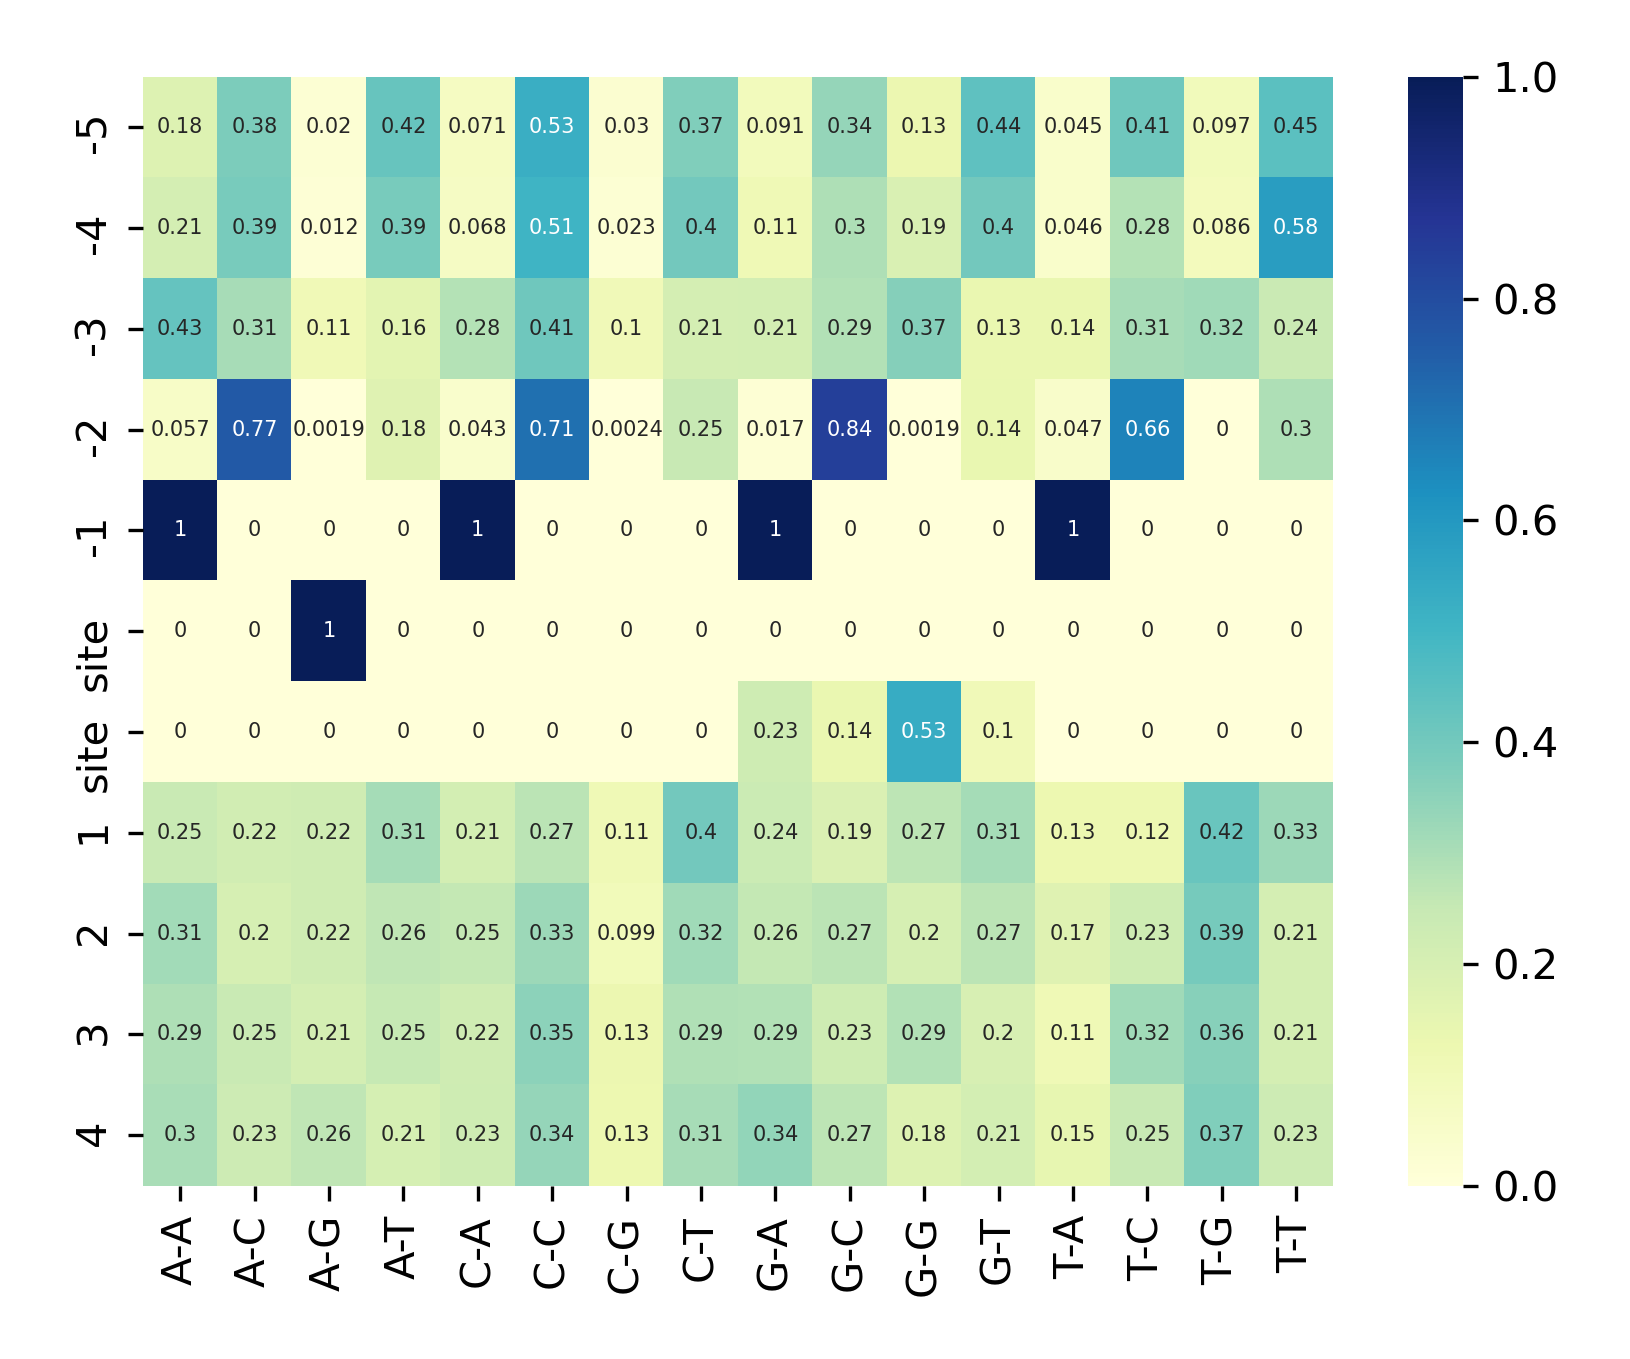
\includegraphics[scale=0.6]{Pics/asheatmap_acceptor.png}}
\caption{Base distribution represented as heatmaps for donor splice sites. \textbf{Top}: single base distribution of positive donor \& negative samples. Aside from two conservative sites GT (labeled with ``site''), Positions (-2, -1, +1, +2, +3) shows additional conservation of adjacent sites of a splice site. For example, it is attractive that the odds reach 84\% of position +3 being a guanine. \textbf{Center}: adjacent base distribution of positive donor \& negative samples which shows the correspondence between bases more clearly compared with the single base heatmaps. \textbf{Bottom}: base distribution of positive acceptor samples. The polypyrimidine tract can be observed (-5, -4, -3) likewise, with the sum of $P(C)$ and $P(T)$ exceeds 80\%, which is part of the powerful acceptor signal. }
\label{fig3}
\end{figure*}

The base distribution of positive samples nicely dovetails with the currently accepted splice site pattern, as shown in Fig. \ref{fig3}, which further proves the validity of our proposed method: the conditional probability matrices are capable of reflecting special functional signals in nucleotide sequences. 

\subsection{Prediction}\label{2.4}

We apply the P matrices above to make judgment of splice sites in unknown sequences. To be specific, we set a sliding window to extract sequences of every available position of the testing set, and score them with a scoring function $S(X)$. For a binary classifier, the scoring formula is a log-odds ratio as: 
\begin{small}
\begin{equation}
S(X) = \ln \displaystyle\frac{P^+(X)}{P^-(X)} 
= \ln \displaystyle\frac{P_0^+[1, N_1]}{P_0^-[1, N_1]} + \sum\limits_{i=2}^\lambda\ln \displaystyle\frac{P^+[i, N_{i-1}, N_i]}{P^-[i, N_{i-1}, N_i]}
\label{eq5}
\end{equation}
\end{small}

Since there is zeros in the probability matrices, we set  $P = 10^{-6}$  to avoid division-by-zero error which, in the meantime, guarantees a higher penalty for a sequence including a $P^+(X) = 0$ site, and vice versa. By this way, we score all sequence txts of the testing set and get the score distributions of donor and acceptor predicting models, as is shown in Fig. \ref{fig4}. The distributions are conducive to the selection of thresholds at the following steps. 

\begin{figure}[htbp]
\centerline{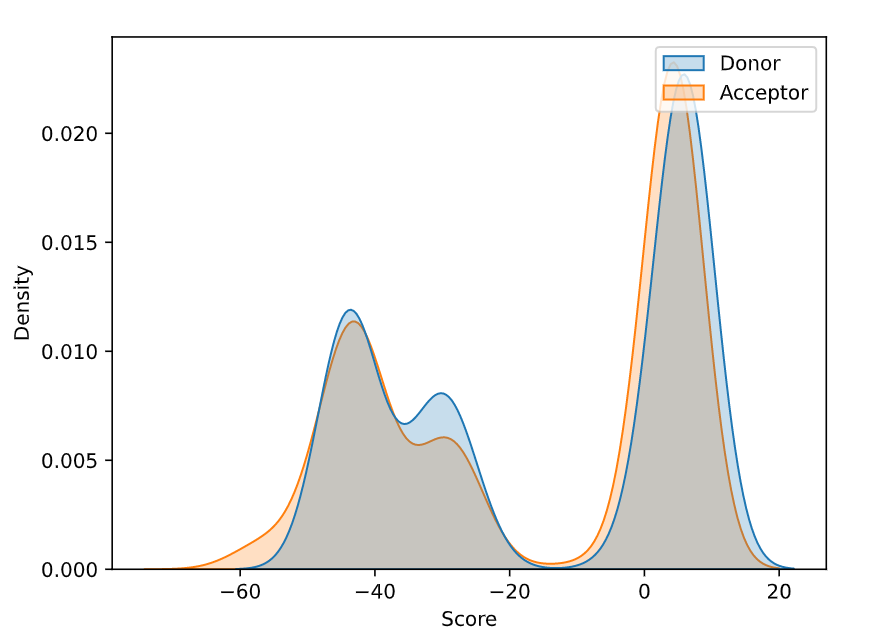
\includegraphics[scale=0.3]{Pics/density.png}}
\caption{Density of sequence scores predicted separately by donor (blue) and acceptor (coral) WAMs. Compared to the histograms Rodger \cite{staden1984computer} provided earlier, there are a lot of low scores in our testing consequence. This is caused by the sliding selection of testing sequences without filtering pseudo ones with the conservative sites on purpose. It can also be observed that low and high scores are widely separated, hence can be easily distinguished. Comparing donor and acceptor scores latitudinally, we can see difference between the sequence pattern of donor and acceptor sites, but it is small enough to allow the acceptor prediction without changing the framework of our approach. }
\label{fig4}
\end{figure}

Transformation from scores to predicting results needs the comparison. We can filter the true positive sites we need from batches of scores by taking different thresholds. It is necessary to exercise caution in selecting the threshold $C$. A large $C$ will exclude potential positive sites, while a small $C$ misclassifies negative sites as positive. Hence an appropriate threshold is a tradeoff based on the specificity and sensitivity of a model. For the threshold optima selection, see \ref{4} for details. 

\section{Experiments}\label{3}

\subsection{Data}\label{3.1}

We conduct our experiment on the eukaryotic gene sequence dataset Kulp \& Reese \cite{reese1997improved} and Burset \& Guigo \cite{burset1996evaluation}. Human genome sequence dataset Kulp \& Reese (KR set) is used as training set which contains 462 sequence text files, each records the name, length, CDS terminal points and the segment. 2,381 donor sites and 2,381 acceptor sites are extracted from the KR set. Vertebrate genome dataset Burset \& Guigo (BG set) is used as testing set which contains 570 sequence text files with a similar format, except for a lack of the sequence length. 

The KR and BG set is open access and you can get the entire dataset at \url{https://www.fruitfly.org/sequence/human-datasets.html} and \url{http://www1.imim.es/databases/genomics96/}. 

\subsection{Metrics}\label{3.2}

Our model accuracy measures are given by \eqref{eq6} -- \eqref{eq12}: 
\begin{gather}
    \text{Precision} = \displaystyle\frac{\text{TP}}{\text{TP} + \text{FP}}\label{eq6} \\
    \text{Recall} = \displaystyle\frac{\text{TP}}{\text{TP} + \text{FN}}\label{eq7} \\
    \text{FPR} = \displaystyle\frac{\text{FP}}{\text{TN} + \text{FP}}\label{eq8} \\
    \text{TPR} = \displaystyle\frac{\text{TP}}{\text{TP} + \text{FN}}\label{eq9} \\
    \text{F1-Score} = \displaystyle\frac{2 \times \text{Precision} \times \text{Recall}}{\text{Precision} + \text{Recall}}\label{eq10}
\end{gather}
where $\text{TP}$, $\text{FP}$, $\text{TN}$, $\text{FN}$ are metrics of the confusion matrix \cite{stehman1997selecting}. Precision-Recall curves and ROC curves \cite{powers2020evaluation}\cite{fawcett2006introduction} are plotted to make the performance of our model more intuitive. We also calculate areas under the curves by: 
\begin{gather}
    \text{AP} = \int_0^1 P(R)\text{d}R = \sum\limits_{i=1}^n P_i\Delta R_i\label{eq11} \\
    \text{AUC} = \int_0^1 T(F)\text{d}F = \sum\limits_{i=1}^n T_i\Delta F_i\label{eq12}
\end{gather}
where $\text{AP}$ summarizes a precision-recall curve as the weighted mean of precisions achieved at each threshold, with the increase in recall from the previous threshold used as the weight \cite{zhu2004recall}. $\text{AUC}$ is equal to the probability that the model will rank a randomly chosen positive sample higher than a randomly chosen negative one (assuming that ``positive'' ranks higher than ``negative''), where $F$ denotes false positive rate and $T$ denotes true positive rate \cite{fawcett2006introduction}. 

\begin{figure*}[htbp]
\centerline{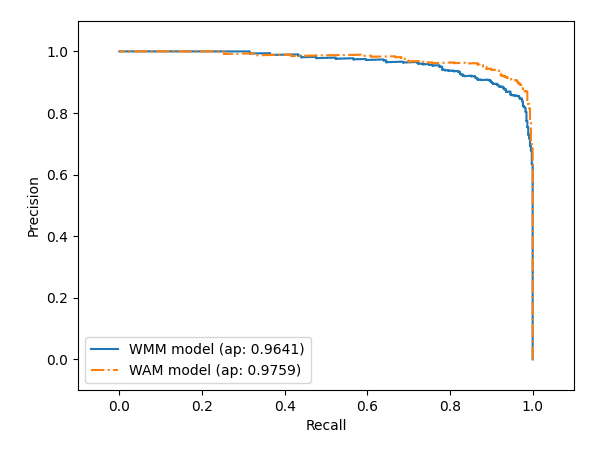
\includegraphics[scale=0.58]{Pics/WMM_WAM_prcurve_donor.png}
    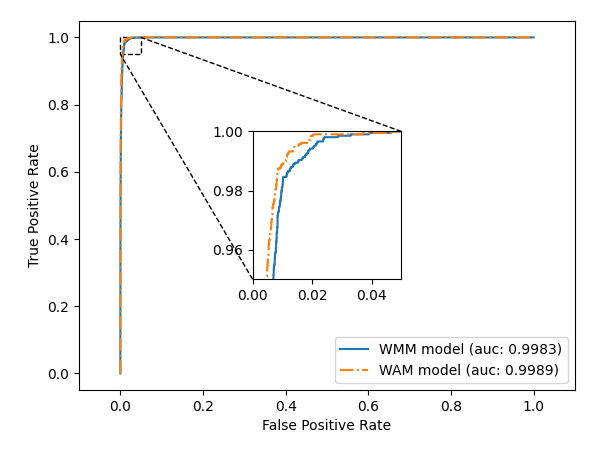
\includegraphics[scale=0.58]{Pics/WMM_WAM_roccurve_donor.png}}
\caption{Measuring WMM \& WAM models on part of the BG set. \textbf{Left}: Precision-Recall curves plotted by using a bunch of thresholds. Average Precision is marked at the figure legend, which represents areas under the P-R curves. Both two models performed well on the given training data with impressive predicting precisions, aside from which WAM model has a much higher AP (0.9759) than WMM (0.9641), which means that WAM predicts fewer false positive results under the circumstance of the correct prediction of the same amount of positive sites. \textbf{Right}: ROC curves with AUC marked at the figure legend, which represents areas under the ROC. The results conforms to P-R curves' as expected, although it's harder to tell the difference between two models. }
\label{fig5}
\end{figure*}

\begin{figure*}[htbp]
\centerline{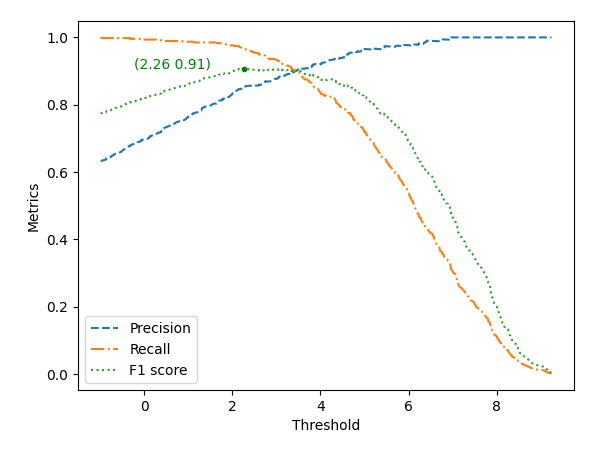
\includegraphics[scale=0.58]{Pics/WMM_threshold_donor.png}
    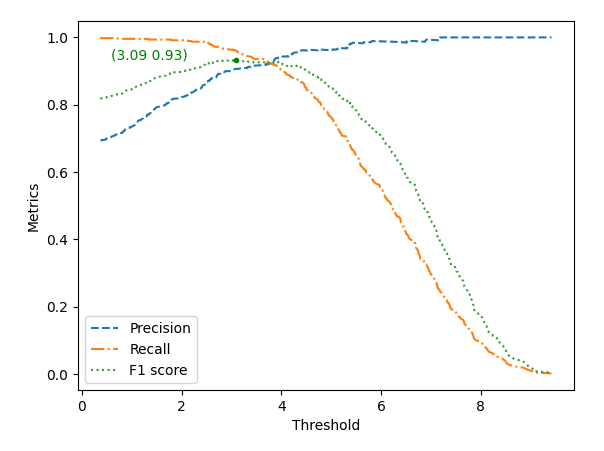
\includegraphics[scale=0.58]{Pics/WAM_threshold_donor.png}}
\caption{Searching for the best thresholds for donor prediction. F1-score \eqref{eq10} is a balanced metric between precision and recall which expresses best performance of models. We have found the maximum F1 points and values for both models: \textbf{left}, WMM, (2.26, 0.91) ; \textbf{right}, WAM, (3.09, 0.93). }
\label{fig6}
\end{figure*}

\subsection{Implementation}\label{3.3}

We encapsulate the WAM model in the class \texttt{Wam} which is derived from the base class \texttt{Base} in \texttt{./Model/basemodel.py}. Additionally, intermediate class \texttt{Ssm} is created for the shared parts of WMM and WAM. Sequences are extracted by \texttt{./Utils/extract.py} and saved temporarily in an \texttt{Sequence} object. All of the statistical graphs involved in this paper are drawn by the scripts in \texttt{./Utils} using Matplotlib \cite{Hunter:2007}, Seaborn \cite{Waskom2021} \& Weblogo, and saved in \texttt{./Pics}. We evaluate the model using Scikit-Learn for confusion matrices, precision-recall pairs and FPR-TPR pairs \cite{pedregosa2011scikit}. These tools saved considerable time for model training and prediction. Models can be easily saved or loaded by methods \texttt{save\_model()} and \texttt{load\_model()}. All the components have their corresponding interface methods provided in the aforementioned classes. For the code implementation details of WAM (also WMM), see \texttt{./Model/wam.py}. 

Training \& Predicting process is operated by Ubuntu 18.04.5 LTS on 16 CPU cores with 2 threads each. The source code is available on GitHub and can be obtained from \url{https://github.com/Newiz430/SplicePredictor}. 

\begin{figure*}[htbp]
\centerline{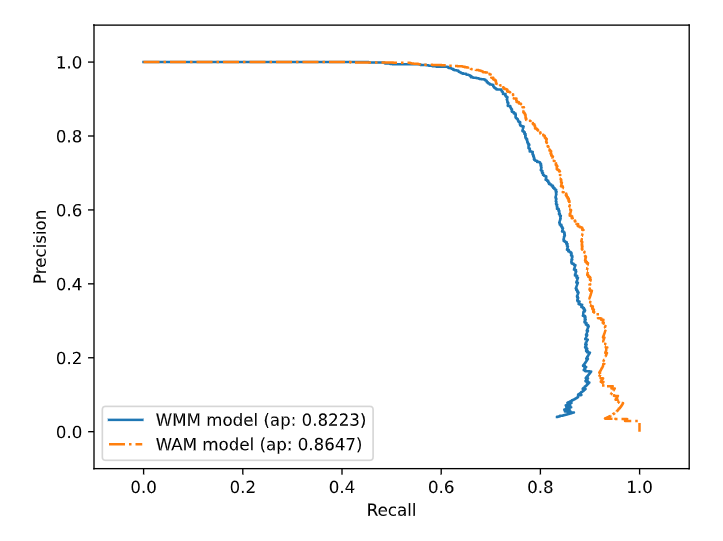
\includegraphics[scale=0.35]{Pics/WMM_WAM_prcurve_acceptor.png}
    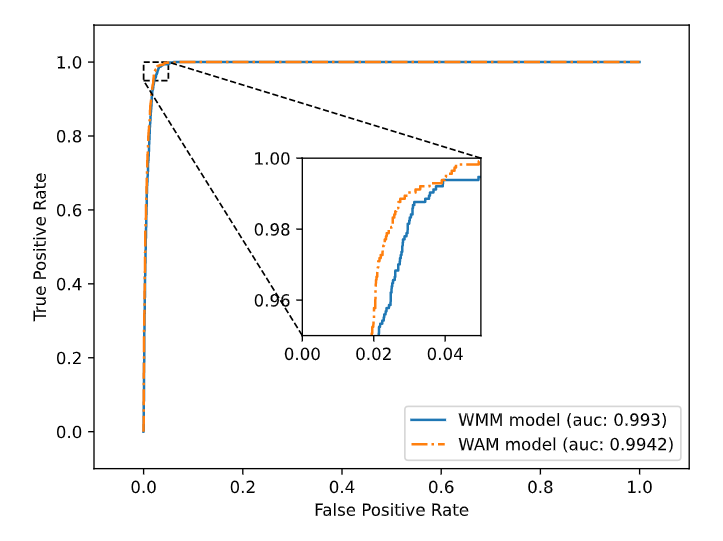
\includegraphics[scale=0.35]{Pics/WMM_WAM_roccurve_acceptor.png}}
\caption{Precision-Recall curves (\textbf{left}) and ROC curves (\textbf{right}) for acceptor signal. WAM Model used for acceptor seems to have a lower predicting ability relative to the one for donor. This can be explained by our hypothesis that adjacent dependencies for acceptor influences the accuracy slighter than donor's. }
\label{fig7}
\end{figure*}

\begin{figure*}[htbp]
\centerline{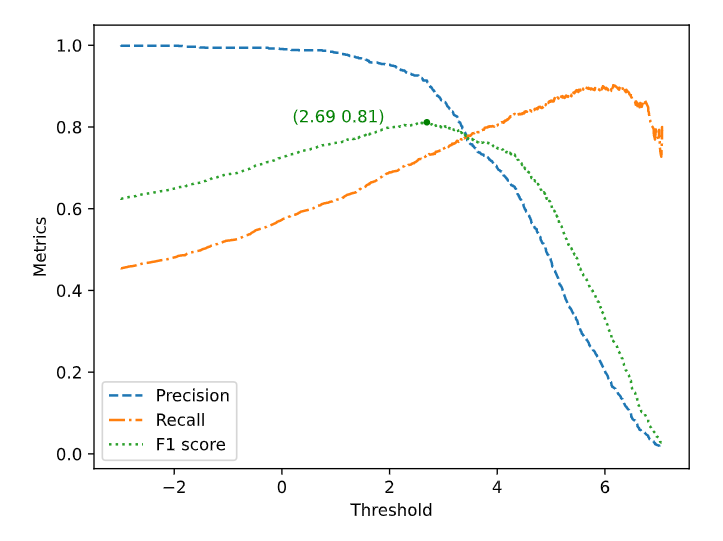
\includegraphics[scale=0.35]{Pics/WMM_threshold_acceptor.png}
    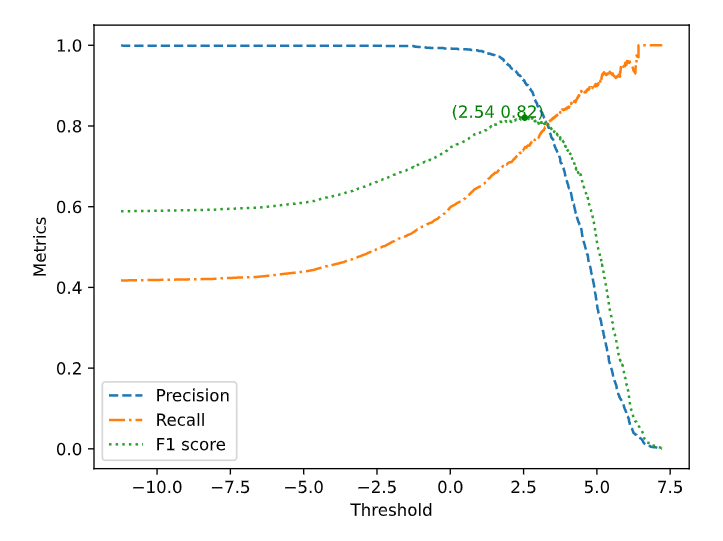
\includegraphics[scale=0.35]{Pics/WAM_threshold_acceptor.png}}
\caption{Searching for the best thresholds for donor prediction. F1-score  \eqref{eq10} is a balanced metric between  precision and recall which expresses best performance of models. We have found the maximum F1 points and values for both models: \textbf{left}, WMM, (2.26, 0.91) ; \textbf{right}, WAM, (3.09, 0.93). }
\label{fig8}
\end{figure*}

\section{Results}\label{4}

\subsection{Donor Site Prediction}\label{4.1}
\emph{Comparison studies. } We compared the performance of our WAM model with the conventional WMM model by Rodger, et al. \cite{staden1984computer} We evaluated two models under a set of different thresholds and the results are shown in Fig. \ref{fig5}. These results validate that WAM outperforms WMM in pattern identification, as  We also found the thresholds with the highest F1 score which indicates the best predicting result, as is shown in Fig. \ref{fig6}. 

We used the training set of the same size and predicting procedure for both two models, and performed them on the same set of testing data with the best threshold Fig. \ref{fig6} pointing out. In Table \ref{tab1}, we present the stats of accuracy for both models. It indicates that WAM improves the overall signal predicting effect within an approximate predicting time. WAM shows a +2.27\% improvement on F1-score from 0.9061 up to 0.9267. 

\subsection{Acceptor Site Prediction}\label{4.2}

We did the same experiment on acceptor sites. Consequences are displayed in Fig. \ref{fig7} -- \ref{fig8} and Table \ref{tab2}. 

\begin{table*}[htbp]
\begin{center}
\begin{threeparttable}
\caption{Performance of WAM Against WMM on Donor Sites\tnote{1}}
\begin{tabular}{lccccc}
\toprule
Method & Precision & Recall (TPR) & FPR & F1-score & Run time(s) \\
\midrule
WMM (threshold = 2.26) & 0.8503 & \textbf{0.9697} & 0.0085 & 0.9061 & \textbf{1.6614} \\
WAM (threshold = 3.09) & \textbf{0.9006} & 0.9543 & \textbf{0.0053} &  \textbf{0.9267} & 1.7940 \\
\bottomrule
\end{tabular}
\begin{tablenotes}
    \footnotesize
    \item[1] The argmax thresholds are assigned to these models to get the best metrics. Run time represents the seconds cost in the predicting step. Same for tables below. 
\end{tablenotes}
\label{tab1}
\end{threeparttable}
\end{center}
\end{table*}

\begin{table*}[htbp]
\begin{center}
\begin{threeparttable}
\caption{Performance of WAM Against WMM on Acceptor Sites}
\begin{tabular}{lccccc}
\toprule
Method & Precision & Recall (TPR) & FPR & F1-score & Run time(s) \\
\midrule
WMM (threshold = 2.69) & 0.7385 & \textbf{0.9038} & 0.0160 & 0.8128 & \textbf{1.3336} \\
WAM (threshold = 2.54) & \textbf{0.7554} & \textbf{0.9038} & \textbf{0.0146} &  \textbf{0.8229} & 1.4286 \\
\bottomrule
\end{tabular}
\label{tab2}
\end{threeparttable}
\end{center}
\end{table*}

For acceptor, WAM shows an +1.24\% improvement on F1-score from 0.8128 up to 0.8229. In a nutshell, data certifies that our model is available for high precision predictions, which neither costs much time nor quantities of computing resources. 

\section{Discussion}

Overall, we formulate and re-implement an application of WAM model by training it on the Kulp \& Reese dataset. We compare its performance against the conventional WMM, and successfully prove its superiority on the accuracy of predicting donor \& acceptor splice sites. 

As a matter of fact, there are still some blemishes in our methods which need to be taken serious consideration. We only sampled a fraction of data for matrix construction thus our model may not attain its best performance with the given training set. We ignored the odds of base indels in signal sequences. We omitted unambiguous bases at the beginning of our work which is likely to be part of the splice site patterns. What's more, we only tried one single feature selection tactic limited by the deadline (our model is actually designed for feature sequences of different lengths as input). 

In the future, we will explore deeper into the frequency-based nucleotide pattern finding methods with better generality, efficiency and practicality, aside from addressing the issues above. 

\section*{Acknowledgment}

This work was supported by Prof. Zhou from College of Life Science \& Technology, Huazhong University of Science and Technology, and Wuhan National Laboratory for Optoelectronics for providing computing resources. Also acknowledge our classmates for helpful suggestions \& corrections. 

\bibliographystyle{unsrt}
\bibliography{references}

\end{document}
